\documentclass{article}

\usepackage{icml2026}
\usepackage{amsmath}
\usepackage{amssymb}
\usepackage{booktabs}
\usepackage{graphicx}

\icmltitlerunning{Positive-Pair Distance for Contrastive Temperature Scheduling}

\begin{document}

\twocolumn[
\icmltitle{Positive-Pair Distance Can Schedule Contrastive Temperature\\ Without a Grid Search}

\begin{icmlauthorlist}
\icmlauthor{Anonymous Authors}{anon}
\end{icmlauthorlist}

\icmlaffiliation{anon}{Anonymous Institution}
\icmlcorrespondingauthor{Anonymous Authors}{anonymous@example.com}

\icmlkeywords{contrastive self-supervised learning, temperature scheduling, kernel density estimation, representation collapse, positive-pair scale scheduling}

\vskip 0.3in
]

\printAffiliationsAndNotice{}

\begin{abstract}
The temperature hyperparameter $\tau$ in InfoNCE controls the quality of contrastive self-supervised representations, but it is typically chosen by grid search rather than by a data-dependent rule. On the unit hypersphere, the cosine-softmax weights coincide with Gaussian kernel weights of variance $\sigma^2=\tau$, so $\sqrt{\tau}$ is exactly the bandwidth of a kernel density estimate over embeddings. This identification recasts temperature selection as bandwidth selection and suggests that useful temperatures are those whose bandwidth matches the scale of meaningful neighborhoods in the embedding space: over-large bandwidths can produce low-rank representations, while over-small bandwidths assign most softmax mass to a small number of neighbors, reducing gradient signal for the rest. We use this view to motivate a positive-pair scale (PPS) schedule that ties $\tau$ to the current positive-pair chord distance. On CIFAR-10 with SimCLR and a ResNet-18 encoder, the PPS schedule avoids collapse and reaches 78.68\% linear-probe accuracy, within 0.47 percentage points of the best completed fixed-temperature sweep, without running a separate sweep.
\end{abstract}

\section{Introduction}

Contrastive self-supervised learning trains visual encoders by bringing augmented views of the same image together and pushing different images apart. The temperature in the InfoNCE denominator controls how sharply the loss weights these pairwise comparisons \citep{oord2018representation,chen2020simple}. In practice, this scalar is often selected by defaults or grid search, even though a full SSL run is expensive and the useful range changes with dataset, architecture, augmentation strength, and batch size.

Temperature is already known to affect hardness awareness, uniformity, and semantic tolerance \citep{wang2020understanding,wang2021understanding,kukleva2023temperature}. Adaptive-temperature methods therefore change $\tau$ over training time, pair similarity, alignment, or per-sample robustness objectives \citep{manna2024dystress,qiu2023not,huang2023model,khaertdinov2022dynamic,wang2024adaptive}. These methods reduce reliance on a single fixed scalar, but their control signals usually treat temperature as a softmax sharpness parameter. The geometric scale imposed on the current embedding distribution remains implicit.

On the unit hypersphere, the cosine-softmax weights used by InfoNCE are exactly Gaussian kernel weights with variance $\sigma^2=\tau$. The temperature therefore determines the neighborhood scale at which positive and negative embeddings are compared. The bandwidth identity connects contrastive training to a classical mean-shift identity for kernel density estimates (KDEs): the score of a Gaussian KDE is the vector from the query point to the kernel-weighted centroid, divided by the bandwidth squared \citep{fukunaga1975estimation,comaniciu2002mean}.

If $\tau=\sigma^2$, selecting temperature becomes selecting bandwidth. The remaining question is what scale the bandwidth should track. We use a label-free local scale already defined by the SSL objective: the distance between two augmented views of the same image. Let $d_{\mathrm{eff}}(t)$ denote this scale, defined as the mean chord distance between the two normalized embeddings of a positive pair. Instead of selecting a fixed temperature before training, set
\begin{equation}
\sigma(t)=\alpha d_{\mathrm{eff}}(t),
\qquad
\tau(t)=\alpha^2 d_{\mathrm{eff}}^2(t).
\label{eq:simple-schedule}
\end{equation}
The rule keeps the kernel bandwidth proportional to the geometry of positive pairs. The intuition is that positive neighborhoods are wide early in training and contract as the encoder learns, and the bandwidth should follow that contraction.

We make three contributions. First, we make explicit the standard equivalence between temperature-scaled cosine softmax on normalized embeddings and Gaussian kernel weights with variance $\sigma^2=\tau$, so that choosing $\tau$ is equivalent to choosing the kernel bandwidth $\sigma=\sqrt{\tau}$ (Section~\ref{sec:kde}). Second, we propose a causal positive-pair scale (PPS) schedule,
\begin{equation*}
\sigma(t)=\alpha\, d_{\mathrm{eff}}(t), \qquad \tau(t)=\alpha^2 d_{\mathrm{eff}}^2(t),
\end{equation*}
where $d_{\mathrm{eff}}(t)$ is the minibatch mean chord distance between two augmented views of the same image (Section~\ref{sec:scheduling}). Third, on CIFAR-10 SimCLR with a ResNet-18 encoder, we show that this schedule reaches 78.68\% linear-probe accuracy, within 0.47 percentage points of the best completed fixed-temperature sweep, while avoiding a separate sweep over $\tau$ (Section~\ref{sec:experiments}).

While the same rule could be stated directly in terms of positive-pair distance, the KDE view gives a cleaner account of why bandwidth is the right quantity to control and connects InfoNCE to mean-shift estimators that have long used kernel bandwidths for the same purpose \citep{fukunaga1975estimation,comaniciu2002mean,hyvarinen2005estimation}.

\section{Related Work}

\paragraph{Contrastive and non-contrastive SSL objectives.}
Contrastive predictive coding, SimCLR, MoCo, CMC, and DCL train encoders through positive and negative comparisons \citep{oord2018representation,chen2020simple,he2020momentum,tian2020contrastive,yeh2022decoupled}. CLIP and SogCLR extend the same denominator-based logic to large-scale multimodal or global-contrastive settings \citep{radford2021learning,yuan2022provable}. Non-contrastive methods such as BYOL, SimSiam, VICReg, Barlow Twins, SwAV, and DINO replace explicit negative comparisons with target networks, distributional constraints, cluster assignments, or teacher-student sharpening \citep{grill2020bootstrap,chen2021exploring,bardes2022vicreg,zbontar2021barlow,caron2020unsupervised,caron2021emerging}.

\paragraph{Geometric diagnostics for representations.}
A parallel line of work characterizes learned embeddings through geometric quantities rather than through the training loss. Alignment and uniformity describe positive-pair closeness and hyperspherical spread \citep{wang2020understanding}; effective rank measures dimensional usage and correlates with downstream accuracy \citep{roy2007effective,garrido2023rankme}; dimensional collapse can appear even with contrastive repulsion \citep{jing2022understanding}. We use these quantities as diagnostics in our experiments.

\paragraph{Adaptive temperature in contrastive learning.}
Kukleva et al. schedule temperature over training time to alternate instance discrimination and group-wise discrimination on long-tailed data \citep{kukleva2023temperature}. DySTreSS makes temperature a bounded function of pairwise similarity, reducing overly strong repulsion for likely false negatives \citep{manna2024dystress}. Qiu et al. derive per-anchor temperatures as dual variables in a KL-constrained distributionally robust objective \citep{qiu2023not}. MACL increases temperature as positive-pair alignment improves \citep{huang2023model}. Other adaptive formulations use external similarity estimators, multi-head uncertainty, or input-dependent uncertainty \citep{khaertdinov2022dynamic,wang2024adaptive,zhang2021temperature}. Existing adaptive methods make temperature dynamic, but the control signal is time, pair similarity, alignment, robustness, or uncertainty. The PPS schedule in Eq.~\eqref{eq:simple-schedule} instead uses a KDE bandwidth matched to the current positive-pair scale.

\paragraph{Score matching and KDE bandwidth.}
Score matching estimates gradients of log densities without computing partition functions \citep{hyvarinen2005estimation}. Denoising autoencoders estimate the score of a Parzen density, and score-based generative models estimate scores across multiple noise levels before sampling with annealed dynamics \citep{vincent2011connection,song2019generative,ho2020denoising}. Recent drifting models use kernel-defined vector fields to move generated samples, and follow-up analysis shows that a Gaussian drift operator is a score difference on smoothed distributions \citep{deng2026drifting,turan2026generative}. That work also studies bandwidth annealing from a spectral perspective. This paper uses the shared KDE identity only to interpret contrastive temperature and to motivate a bandwidth schedule tied to representation geometry.

\section{Temperature as KDE Bandwidth}\label{sec:kde}

On the unit hypersphere, the cosine-softmax weights in InfoNCE are exactly Gaussian kernel weights — so choosing $\tau$ is equivalent to choosing the bandwidth of a kernel density estimate over embeddings.

Let $f_\theta(x)\in\mathbb{S}^{D-1}$ be a normalized embedding. For an anchor $z_i$ and another embedding $z_j$,
\begin{equation}
z_i^\top z_j
=
1-\frac{1}{2}\|z_i-z_j\|^2 .
\end{equation}
The InfoNCE softmax factor therefore satisfies
\begin{equation}
\exp(z_i^\top z_j/\tau)
=
\exp(1/\tau)
\exp\!\left(-\frac{\|z_i-z_j\|^2}{2\tau}\right).
\end{equation}
The constant $\exp(1/\tau)$ cancels inside the normalized softmax. Hence the practical temperature $\tau$ equals the Gaussian KDE variance $\sigma^2$:
\begin{equation}
\tau=\sigma^2, \qquad \sigma=\sqrt{\tau}.
\end{equation}

For anchor $i$, define positive and negative kernel weights
\begin{equation}
w_j^+
=
\frac{\exp(-\|z_i-z_j\|^2/(2\sigma^2))}
{\sum_{k\in P_i}\exp(-\|z_i-z_k\|^2/(2\sigma^2))},
\quad j\in P_i,
\end{equation}
and analogously $w_k^-$ for $k\in N_i$. These weights define positive and negative centroids
\begin{equation}
\mu^+(i)=\sum_{j\in P_i}w_j^+z_j,
\qquad
\mu^-(i)=\sum_{k\in N_i}w_k^-z_k.
\end{equation}
The Gaussian mean-shift identity gives
\begin{equation}
\nabla_z\log\hat p_\sigma(z)
=
\frac{\mu_\sigma(z)-z}{\sigma^2}.
\end{equation}
Subtracting the positive and negative KDE scores yields the local score-ratio direction
\begin{equation}
\nabla_z\log\frac{\hat p^+(z)}{\hat p^-(z)}
\bigg|_{z=z_i}
=
\frac{\mu^+(i)-\mu^-(i)}{\sigma^2}.
\end{equation}
The vector $V(i)=\mu^+(i)-\mu^-(i)$ is therefore a KDE diagnostic of the positive-negative contrast at the bandwidth selected by $\tau$.

\section{Positive-Pair Scale (PPS) Scheduling}
\label{sec:scheduling}

Choosing $\sigma$ chooses which neighbors receive non-negligible kernel weight. A fixed schedule changes this scale as a function of training time. The PPS schedule ties bandwidth to a label-free quantity that is available during training: we compute it online from the previous minibatch, and it corresponds to the positive-pair neighborhood the SSL objective explicitly preserves. The intuition is that positive neighborhoods are wide early in training because the encoder has not yet condensed them, and they contract as training proceeds, so the bandwidth should follow that contraction rather than a fixed time profile.

The local scale used here comes from positives because augmentations define the most reliable unlabeled neighborhood: two views originate from the same image and are explicitly trained to remain close. Negatives provide contrast, but they do not define a clean local structure without labels because minibatch negatives can include false negatives or semantically similar samples. In a general multi-positive notation, the positive local scale is the anchor-to-positive-centroid distance
\begin{equation}
d_{\mathrm{pos}}(i,t)=\|\mu^+(i,t)-z_i(t)\|.
\end{equation}
In two-view SimCLR, each anchor has one positive view, so the positive centroid degenerates to that view. For normalized embeddings $z_i^{(1)}$ and $z_i^{(2)}$, the statistic used in our experiments is therefore
\begin{equation}
d_{\mathrm{eff}}(t)
=
\mathbb{E}_i\|z_i^{(1)}-z_i^{(2)}\|
=
\mathbb{E}_i\sqrt{2-2(z_i^{(1)})^\top z_i^{(2)}} .
\end{equation}
The statistic is a label-free proxy for the local neighborhood scale that SimCLR explicitly trains to preserve. The PPS schedule sets the next temperature according to Eq.~\eqref{eq:simple-schedule}. In implementation, the statistic is computed on one minibatch and applied to the next minibatch. The one-step delay keeps the schedule causal and avoids an additional forward pass.

\section{Experiments}\label{sec:experiments}

All completed experiments use SimCLR with a ResNet-18 encoder on CIFAR-10, batch size 256, projection dimension 128, learning rate 0.05, weight decay $5\times10^{-4}$, Gaussian KDE diagnostics, and 100 epochs. The augmentation recipe is: random resized crop with scale $0.2$--$1.0$, color jitter with strength $0.4$ applied at probability $0.8$, random grayscale at probability $0.2$, and random horizontal flip (no Gaussian blur). The downstream metric is linear-probe accuracy on frozen features, with $k$-NN accuracy, effective rank, and collapse fraction as diagnostic metrics.

\paragraph{Fixed-temperature sweep.}
The fixed sweep shows the expected intermediate-bandwidth behavior. Extremely small temperature underfits or collapses: $\tau=0.01$ gives 62.28\% linear-probe accuracy and collapse fraction 0.978. Extremely large temperature also degrades the representation: $\tau\approx2.0$ gives 70.76\% linear-probe accuracy and effective rank 9.01. The best completed fixed run is $\tau\approx0.206$, with 79.15\% linear-probe accuracy, 83.29\% $k$-NN accuracy, and effective rank 65.35.

\begin{figure}[t]
\centering
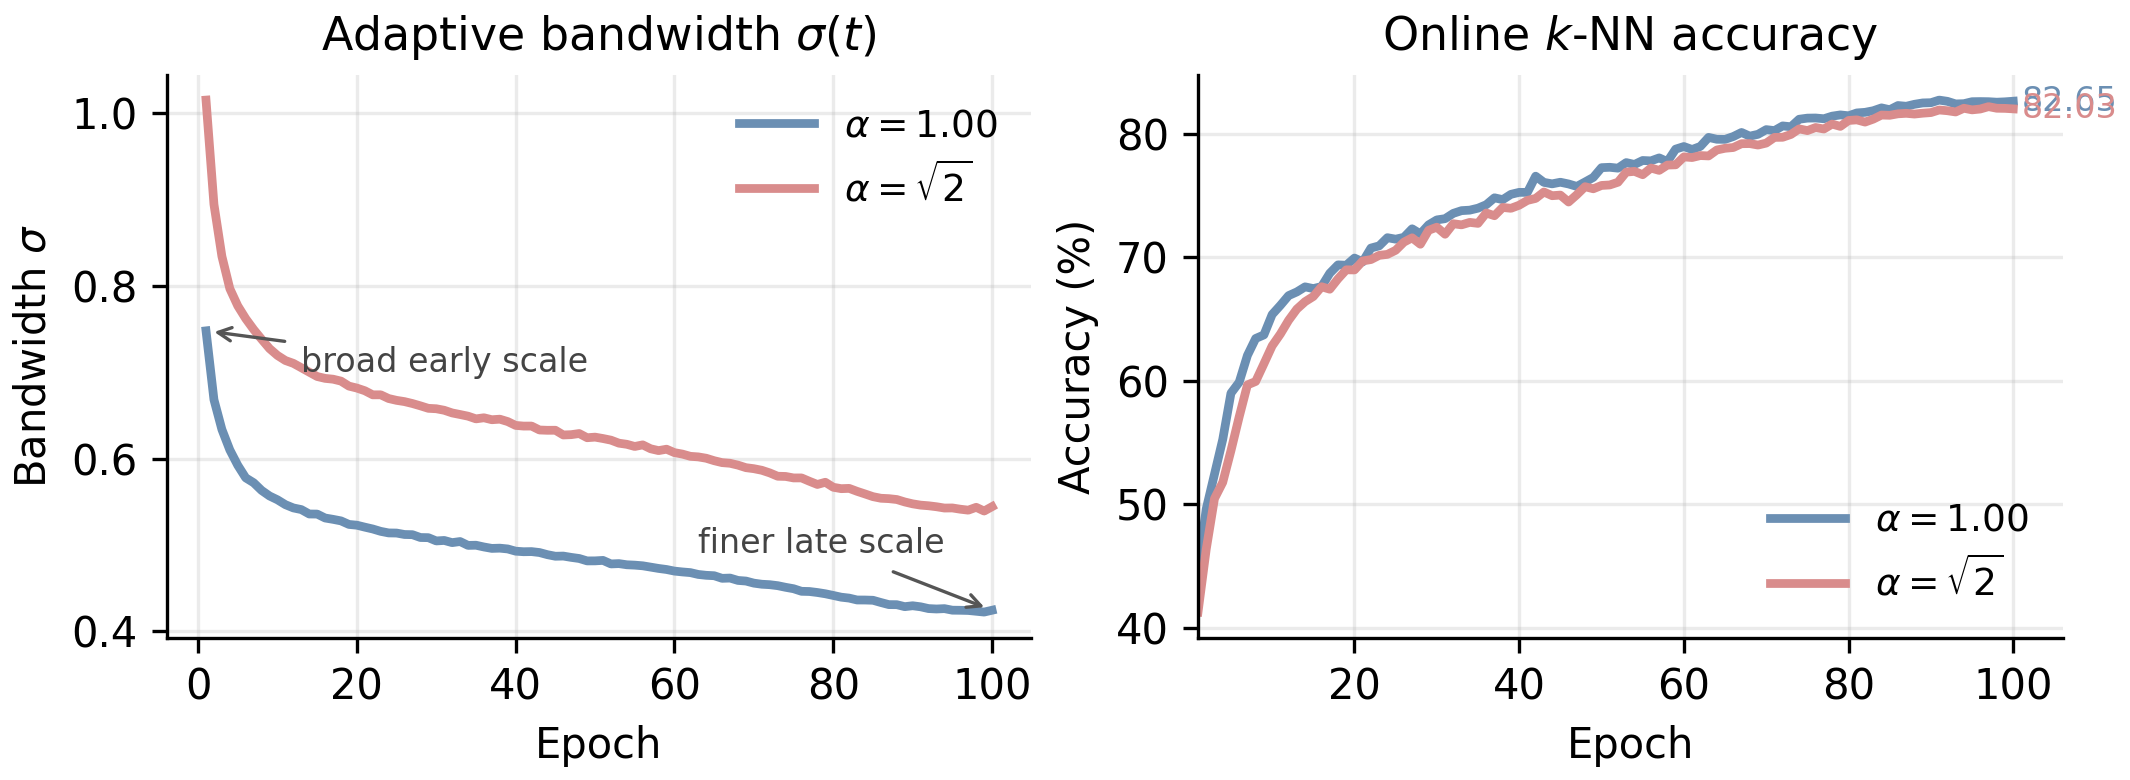
\includegraphics[width=\linewidth]{figures/figure1_adaptive_bandwidth_accuracy.png}
\caption{PPS bandwidth and online accuracy on CIFAR-10 SimCLR. The measured bandwidth starts large and decreases as the positive-pair scale contracts, while $k$-NN accuracy rises. Early training uses a broader neighborhood, and later training resolves a finer local geometry — the PPS schedule follows this natural contraction.}
\label{fig:adaptive-bandwidth-accuracy}
\end{figure}

\paragraph{PPS schedule.}
The experiment evaluates two scale factors of order one, $\alpha=1.0$ and $\alpha=\sqrt{2}$, to test whether the positive-pair scale can reduce the need for a fixed-temperature sweep without introducing a large additional hyperparameter search. The PPS schedule eliminates the temperature sweep: $\alpha=\sqrt{2}$ reaches 78.68\% linear-probe accuracy, within 0.47 percentage points of the best completed fixed run ($\tau\approx0.206$, 79.15\%), while $\alpha=1.0$ reaches 78.41\%. Both runs achieve near-zero collapse fraction ($1.0\times10^{-5}$) without any fixed-temperature search. The trade-off is a roughly 0.5 percentage point gap relative to the sweep-optimum; the benefit is the complete removal of that sweep.

\begin{table}[t]
\caption{Completed CIFAR-10 SimCLR runs. The PPS schedule reaches within 0.47 pp of the best fixed-temperature sweep without running a separate sweep.}
\label{tab:cifar-results}
\centering
\begin{tabular}{lccc}
\toprule
Run & Linear & $k$-NN & Eff. rank \\
\midrule
Best fixed $\tau\approx0.206$ & 79.15 & 83.29 & 65.35 \\
PPS $\alpha=1.0$ & 78.41 & 82.65 & 62.90 \\
PPS $\alpha=\sqrt{2}$ & 78.68 & 82.03 & 41.97 \\
\bottomrule
\end{tabular}
\end{table}

\section{Discussion}

The schedule uses $d_{\mathrm{eff}}$ because positive pairs provide the cleanest unlabeled local scale in two-view SimCLR. Negative neighborhoods, class-center estimates, score-ratio drift, or higher-order local statistics could define other scales. The current experiments show the narrower claim that the positive-pair chord distance is stable enough to keep training inside the non-collapsed bandwidth regime for two order-one scale factors.

Here, the drift vector $V=\mu^+-\mu^-$ serves as a diagnostic score-ratio field; the mean-shift identity explains why this diagnostic is tied to the current bandwidth and whether positive and negative neighborhoods exert a nonzero local signal. This vector is the same mean-shift type object used as a drifting field in recent generative work \citep{deng2026drifting,turan2026generative}, though here the two distributions are positive and negative embedding neighborhoods rather than generated and data distributions. Preliminary controllers based on more detailed local formulas were unstable, which suggests that a local statistic can be mathematically meaningful as a measurement while still being impractical as an online assignment rule.

\paragraph{Kernel choice.}
This paper tunes one parameter of one kernel: the bandwidth of the Gaussian that sits, implicitly, inside InfoNCE. The KDE view opens a second axis that the standard fixed-softmax formulation does not expose, namely the kernel shape itself — the Gaussian is one of many coherent choices that fit the same $\mu^+,\mu^-$ machinery.

\paragraph{Limitations.}
The evidence in this paper is bounded in four ways. First, all runs are on CIFAR-10 with a ResNet-18 encoder; the study required repeated full training runs, so transfer to larger images, larger architectures, and multimodal contrastive objectives such as CLIP is not tested. Second, only SimCLR is studied; momentum-encoder methods (MoCo) and non-contrastive methods (BYOL, VICReg) use the temperature differently and would need a separate treatment. Third, the schedule introduces a new scale factor $\alpha$; we evaluate only $\alpha\in\{1,\sqrt{2}\}$, which is enough to suggest moderate robustness but not enough to characterize the full sensitivity. Fourth, the PPS schedule reaches within 0.47 percentage points of the best fixed $\tau\approx0.206$; the benefit is the removal of a per-setting sweep rather than an improvement over the sweep-optimum.

\section{Conclusion}

For normalized embeddings, the InfoNCE cosine softmax is equivalent to Gaussian kernel weighting with variance $\tau$, so $\sqrt{\tau}$ can be interpreted as a KDE bandwidth. This equivalence explains why temperature controls representation quality and motivates the PPS schedule, $\tau(t)=\alpha^2d_{\mathrm{eff}}^2(t)$, based on the current positive-pair scale. CIFAR-10 experiments show that the PPS schedule avoids collapse and reaches 78.68\% linear-probe accuracy, within 0.47 percentage points of the best completed fixed-temperature sweep, without running a separate sweep. The same scale factor works for both $\alpha=1$ and $\alpha=\sqrt{2}$, suggesting moderate robustness to the choice of $\alpha$ in this range.

\bibliography{references}
\bibliographystyle{icml2026}

\clearpage
\onecolumn
\appendix
\section{Additional Training Diagnostics}

The panels below show how the fixed and PPS schedules differ in training dynamics.

\begin{figure}[!ht]
\centering
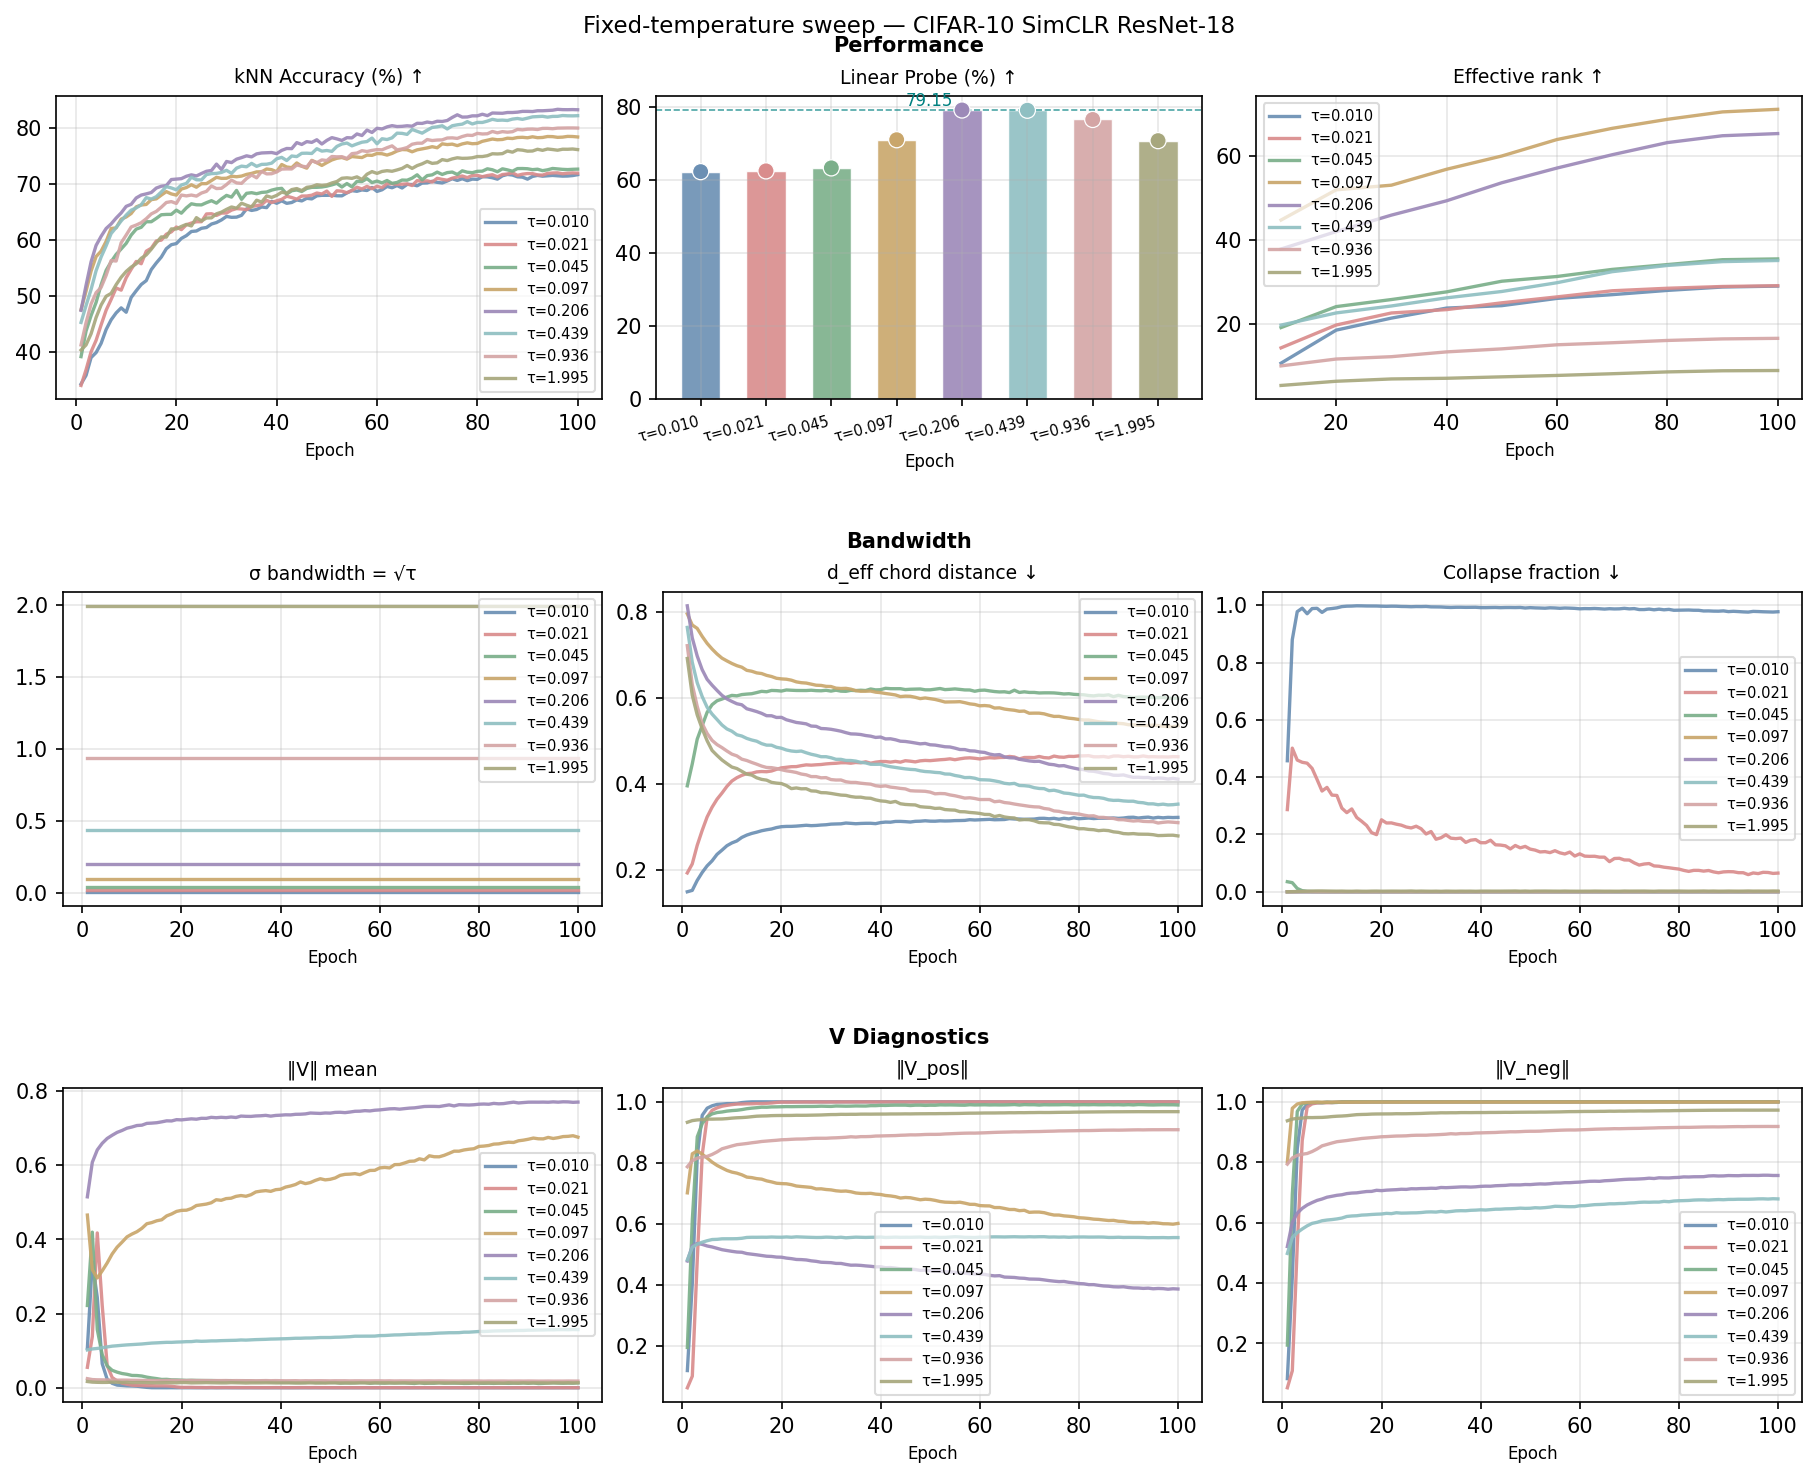
\includegraphics[width=\linewidth]{figures/paper_fig_sweep.png}
\caption{Fixed-temperature sweep on CIFAR-10 SimCLR. The best downstream performance appears in an intermediate bandwidth regime. Very small temperatures can drive the contrastive loss down while producing poor geometry, whereas very large temperatures smooth the pairwise comparisons too strongly.
\protect\\ $k$-NN Accuracy / Linear Probe -- downstream performance peaks at an intermediate $\tau$.
\protect\\ $d_{\mathrm{eff}}$ chord distance and $\sigma$ bandwidth -- shows the neighborhood scale implied by each fixed $\tau$.
\protect\\ Collapse fraction and Effective rank -- geometric quality diagnostics; collapse is severe at $\tau=0.01$ and rank degrades at large $\tau$.
\protect\\ $\|V\|$ mean, $\|V_{\mathrm{pos}}\|$, $\|V_{\mathrm{neg}}\|$ -- drift-vector components indicating the strength of the local positive-negative contrast at each bandwidth.}
\label{fig:appendix-fixed-sweep}
\end{figure}

\begin{figure}[!ht]
\centering
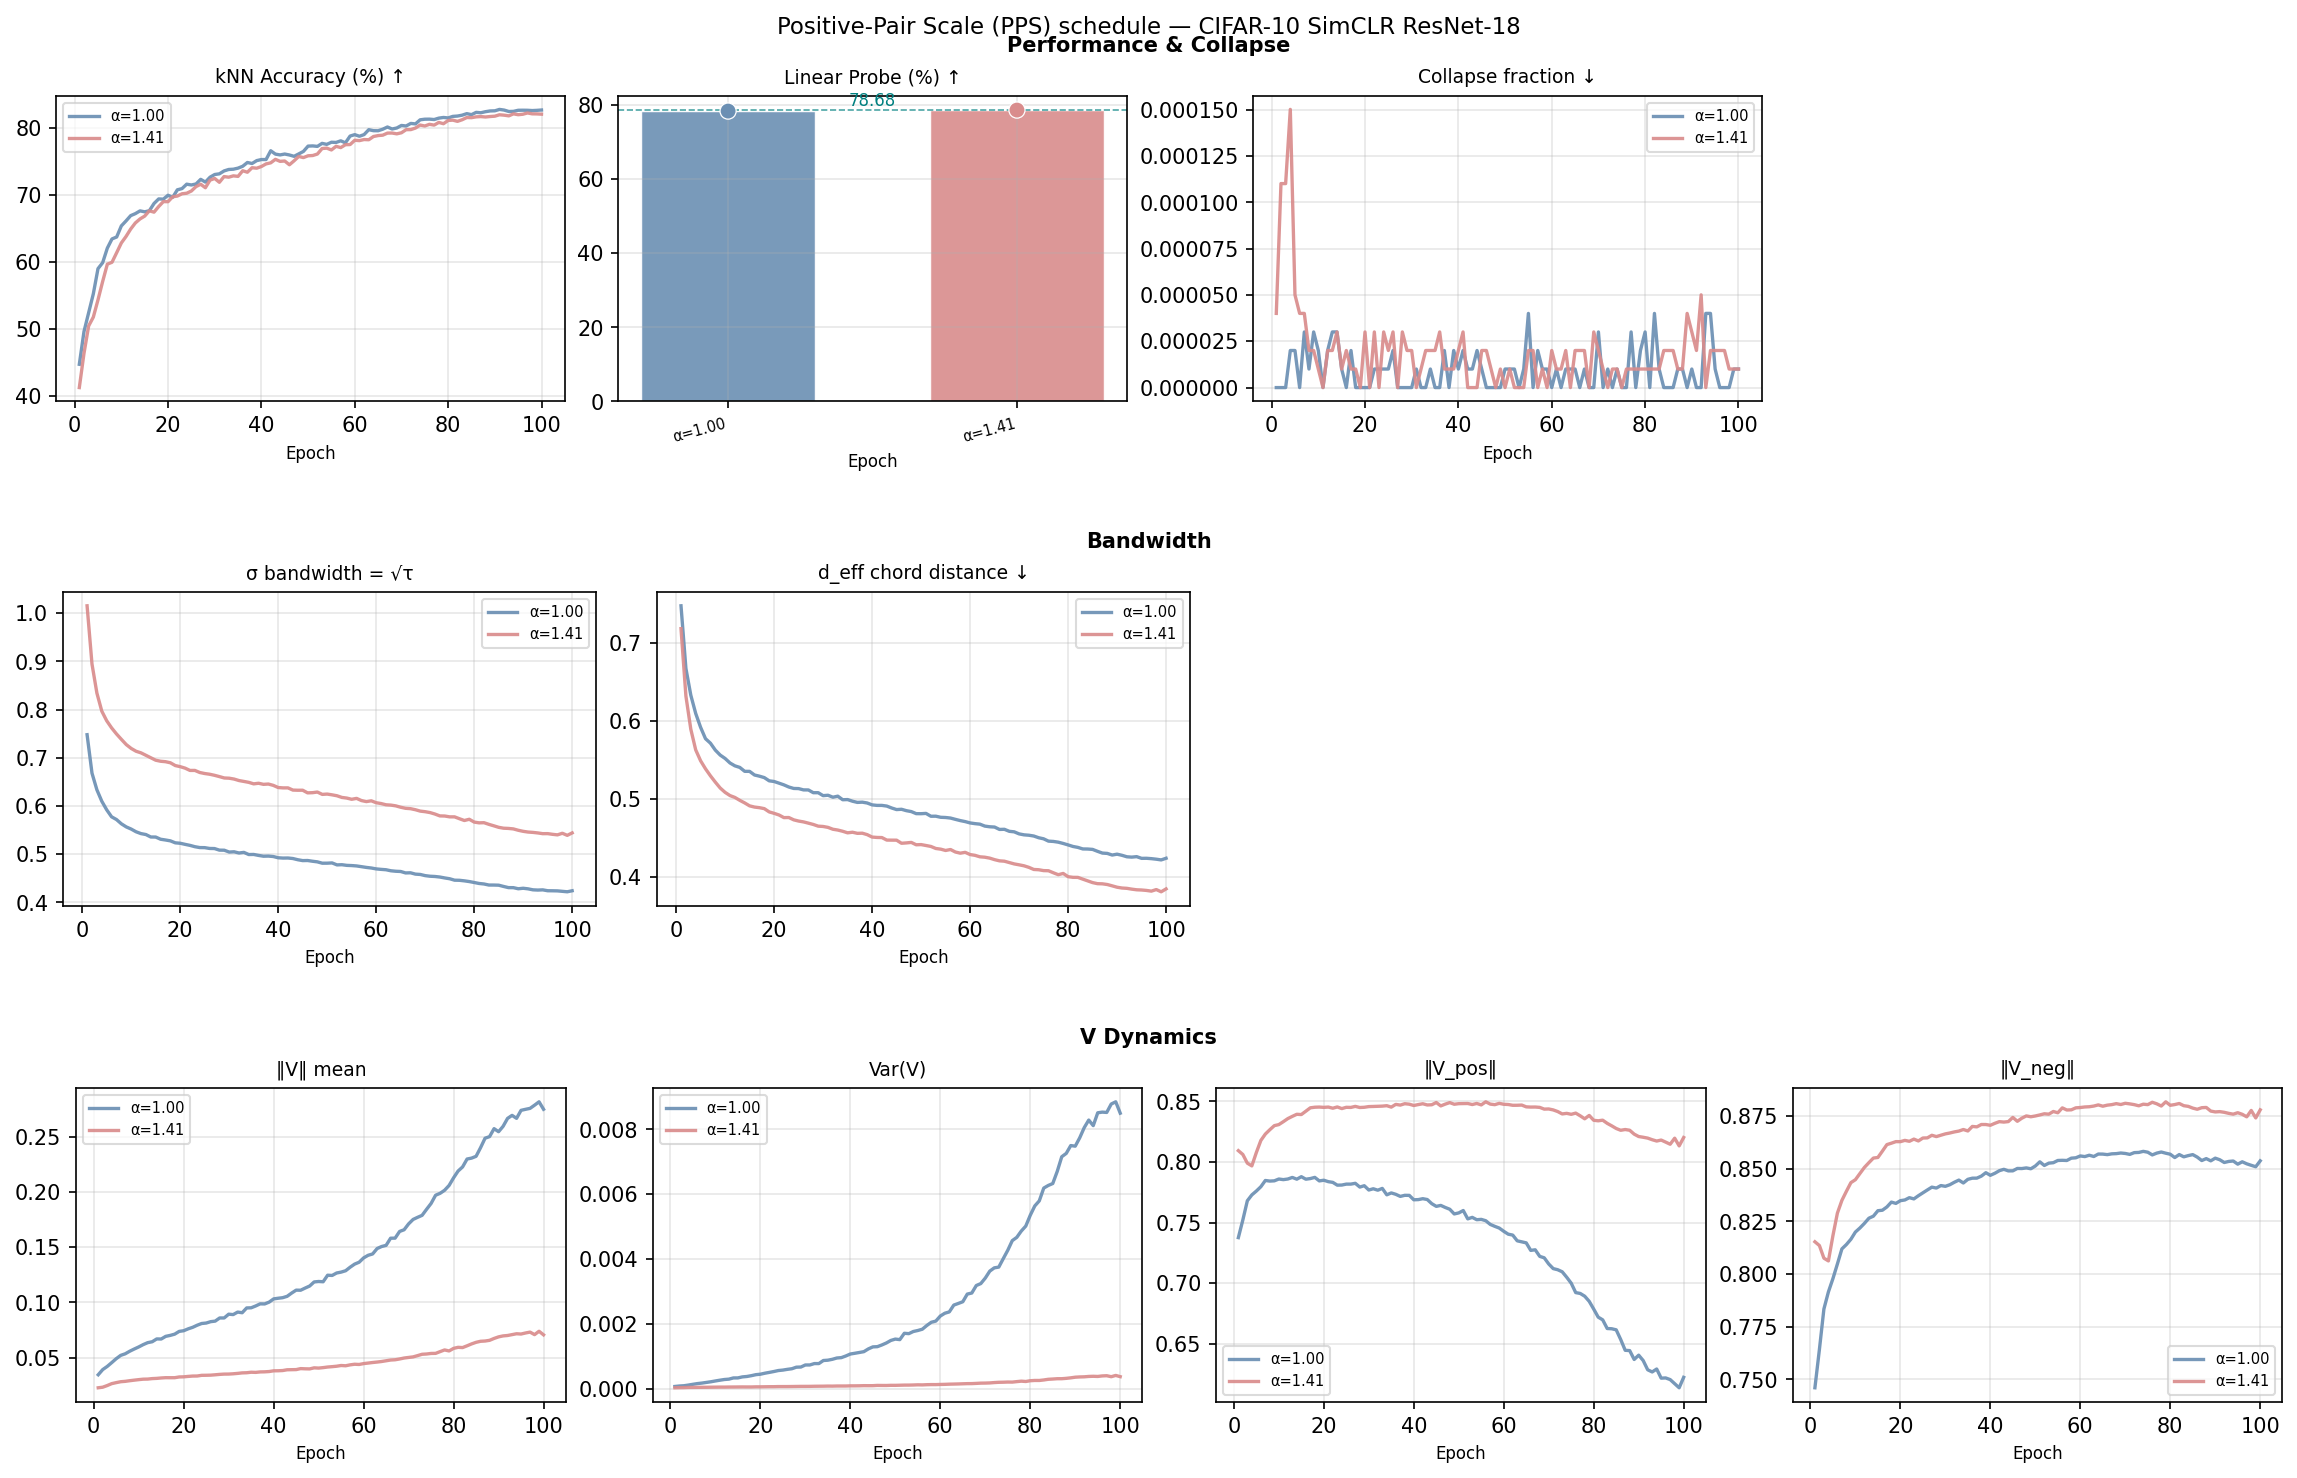
\includegraphics[width=\linewidth]{figures/paper_fig_pps.png}
\caption{PPS schedule with $\alpha=1.0$ and $\alpha=\sqrt{2}$. The scale factor $\alpha$ sets $\sigma(t)=\alpha d_{\mathrm{eff}}(t)$ and $\tau(t)=\alpha^2d_{\mathrm{eff}}^2(t)$.
\protect\\ Linear probe / $k$-NN accuracy -- both settings reach similar downstream accuracy near the sweep-optimum.
\protect\\ $d_{\mathrm{eff}}$ chord distance and $\sigma$ bandwidth -- bandwidth tracks positive-pair scale, confirming the bandwidth contraction over training.
\protect\\ Collapse fraction -- remains near zero throughout training for both scale factors.
\protect\\ $\|V\|$ mean and Var$(V)$ -- drift-vector magnitude and variance; the smaller scale factor produces a larger and noisier drift signal.
\protect\\ $\|V_{\mathrm{pos}}\|$ and $\|V_{\mathrm{neg}}\|$ -- attractive and repulsive components of the local score-ratio field.}
\label{fig:appendix-adaptive-sweep}
\end{figure}

\end{document}
